\begin{frame}
  \frametitle{Distance vs.\ norm}
  %% \framesubtitle{}

  \begin{columns}[T]
    \begin{column}{50mm}
      \begin{itemize}
      \item<1-> Intuitively, \h{distance} $\dist{\vu}{\vv}$ should correspond to
        \h{length} $\norm{\vu-\vv}$ of displacement vector $\vu - \vv$
        \begin{itemize}
        \item $\dist{\vu}{\vv}$ is a \h{metric}
        \item $\norm{\vu-\vv}$ is a \h{norm}
        \item $\norm{\vu} = \bigdist{\vu}{\vnull}$
        \end{itemize}
      \item<2-> Such a metric is always \h{translation-invariant}%
        \gap
      \item<3-> $\dist[p]{\vu}{\vv} = \norm[p]{\vv-\vu}$
      \end{itemize}
    \end{column}
    \begin{column}{50mm}
      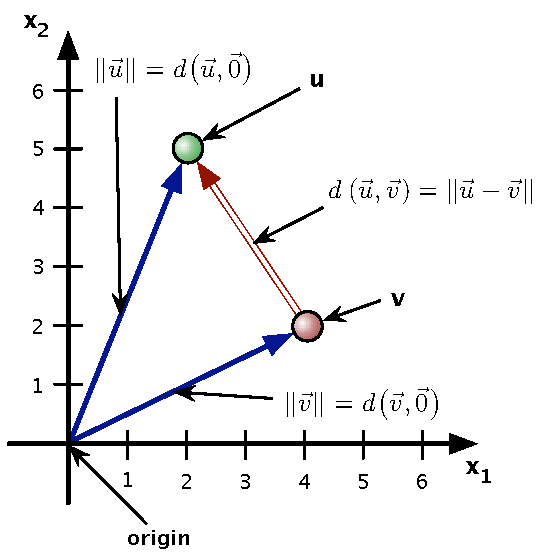
\includegraphics[width=50mm]{img/2_distance_norm}
    \end{column}
  \end{columns}

  \begin{itemize}
  \item<3-> \h{Minkowski $p$-norm} for $p\in [1,\infty]$:
    \[
    \norm[p]{\vu} \coloneq \bigl(\abs{u_1}^p + \dots + \abs{u_n}^p\bigr)^{1/p}
    \]
  \end{itemize}
\end{frame}

\begin{frame}
  \frametitle{Norm: a measure of length}
  %% \framesubtitle{}

  \begin{itemize}
  \item A general \h{norm} $\norm{\vu}$ for the length of a vector $\vu$ must
    satisfy the following \h{axioms}:
    \begin{itemize}
    \item $\norm{\vu} > 0$ for $\vu \neq \vnull$
    \item $\norm{\lambda\vu} = \abs{\lambda}\cdot \norm{\vu}$
      (\h{homogeneity}, not req'd for metric)
    \item $\norm{\vu + \vv} \leq \norm{\vu} + \norm{\vv}$
      (\h{triangle inequality})
    \end{itemize}
    \pause\gap
  \item every norm defines a translation-invariant metric
    \[ \dist{\vu}{\vv} \coloneq \norm{\vu - \vv} \]
  \end{itemize}
\end{frame}

\begin{frame}
  \frametitle{Norm: a measure of length}
  %% \framesubtitle{}

  \begin{columns}[T]
    \begin{column}{50mm}
      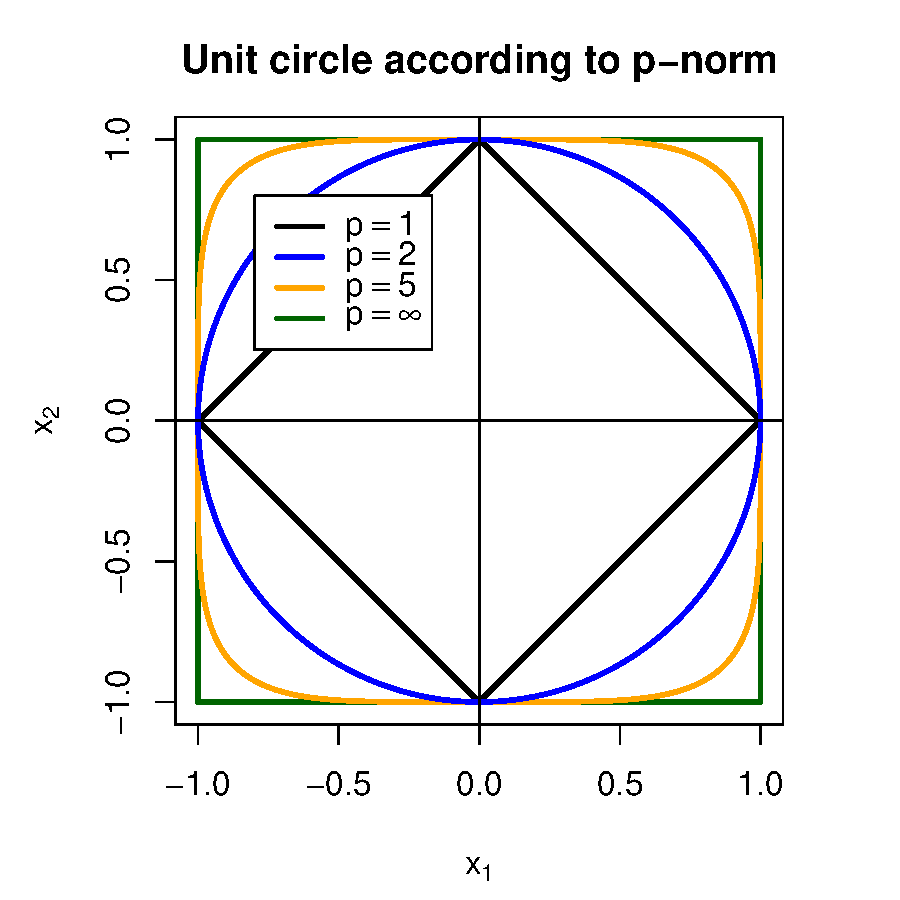
\includegraphics[width=50mm]{img/2_p_norms}
    \end{column}
    \begin{column}{50mm}
      \begin{itemize}
       \item Visualisation of norms in $\setR^2$ by plotting \h{unit
           circle} for each norm, i.e.\ points $\vu$ with $\norm{\vu}=1$
       \item Here: $p$-norms $\norm[p]{\cdot}$ for different values of $p$%
         \pause
       \item Triangle inequality $\iff$ unit circle is \h{convex}
       \item This shows that $p$-norms with $p < 1$ would violate the triangle
         inequality
      \end{itemize}
    \end{column}
  \end{columns}
  \pause%
  \begin{itemize}
  \item Consequence for DSM: $p \gg 2$ ``favours'' small differences in many
    coordinates, $p \ll 2$ differences in few coordinates
  \end{itemize}
\end{frame}

\begin{frame}
  \frametitle{Which metric should I use?}
  %% \framesubtitle{}

  \begin{itemize}
  \item Choice of metric or norm is one of the parameters of a DSM
    \pause
  \item Measures of \h{distance} between points:
    \begin{itemize}
    \item intuitive Euclidean norm $\norm[2]{\cdot}$
    \item ``city-block'' Manhattan distance $\norm[1]{\cdot}$
    \item maximum distance $\norm[\infty]{\cdot}$
    \item general Minkowski $p$-norm $\norm[p]{\cdot}$
    \item and many other formulae \ldots
    \end{itemize}
    \pause
  \item Measures of the \h{similarity} of arrows:
    \begin{itemize}
    \item ``cosine distance'' $\; \sim \ u_1 v_1 + \dots + u_n v_n$
    \item Dice coefficient (matching non-zero coordinates)
    \item and, of course, many other formulae \ldots
    \itemhand these measures determine \h{angles} between arrows
    \end{itemize}
    \pause
  \item Similarity and distance measures are equivalent!
    \begin{itemize}
    \item[\hand] I'm a fan of the Euclidean norm because of its intuitive
      geometric properties (angles, orthogonality, shortest path, \ldots)
    \end{itemize}
  \end{itemize}
\end{frame}

%%% Local Variables: 
%%% mode: latex
%%% TeX-master: "../../workspace"
%%% End: 
